%% This is an example first chapter.  You should put chapter/appendix that you
%% write into a separate file, and add a line \include{yourfilename} to
%% main.tex, where `yourfilename.tex' is the name of the chapter/appendix file.
%% You can process specific files by typing their names in at the 
%% \files=
%% prompt when you run the file main.tex through LaTeX.
\chapter{Implementation and Results}
During the exploration and implementation of the Pedestrian intention prediction pipeline, SSD was chosen as the first block which acts as Pedestrian detector. In this chapter, how SSD was trained on large dataset, acquisition of data set and several aspect of Machine learning and Deep learning shall be discussed.

\section{Data Acqusition}
Challenges are there while just considering image data, the verities of image sources for example we can get photos that are taken by professionals, synthetic photos drawn by image generators and real life photos that we see and capture in our day to day life. So the results of these benchmarks and 
observation across these aforementioned classes of data set does not transfer to the other scenarios.
As recommended always for machine learning tasks, we should consider real data as close as possible to the environment where the designed system is expected to work. And luckily there exist some excellent data set in the public domain. I chose Caltech Data set \cite{dollar2009pedestrian}, which is one of the latest data set available in the public till today. 

\newpara
This data set contains highly annotated video, recorded from a moving vehicle in a normal trafic situation. It contains pedestrians vary largely in appearance, pose and scale. It also includes occlusion information. It contains close to 10 hours of recording at 30 fps with a video resolution 640 x 480. As seen and mentioned by the authors the overall image quality lower than that of same image resolution. The data set includes ~350,000  pedestrian bounding boxes (BB) labeled in 250,000frames and remains the largest such data set to  date. As already mentioned by \cite{walk2010new} Caltech data set is difficult for various reasons.

\begin{itemize}
	\setlength\itemsep{-1em}
	\item Many small pedestrians
	\item realistic occlusion frequency
	\item image quality is poor
	\item includes blur
	\item visible JPEG artifacts
\end{itemize}

\subsection{Data preparation}
After the video data got acquired, with help of a publicly available python project \cite{shuntasaito2015}, the original annotations in \textit{MATLAB} compatible \textit{vbb} format is converted to a JSON structure for easier consumption. The generated json file further processed and required data is extracted into a csv file using a python script located at \url{ https://github.com/Kalinga/ML/blob/master/ssd_keras_caltech/json_anno_csv_conversion.ipynb}. As mentioned by \cite{dollar2009pedestrian} the video set from 00-05 is expected for training purpose and 06-10 is for testing purpose.

In the Caltech data group of people are separately label as \textit{people}. With the intention, the ML model should learn individual person and identify persons rather than people, when there are several persons close by, i decided to remove \textit{people} class label from the training data set. And also the number of samples for \textit{people} and \textit{person} was disproportionately varying. This was another reason to exclude \textit{people }label from  the training. The frequency for the both classes are shown as below.

\begin{figure}[H]
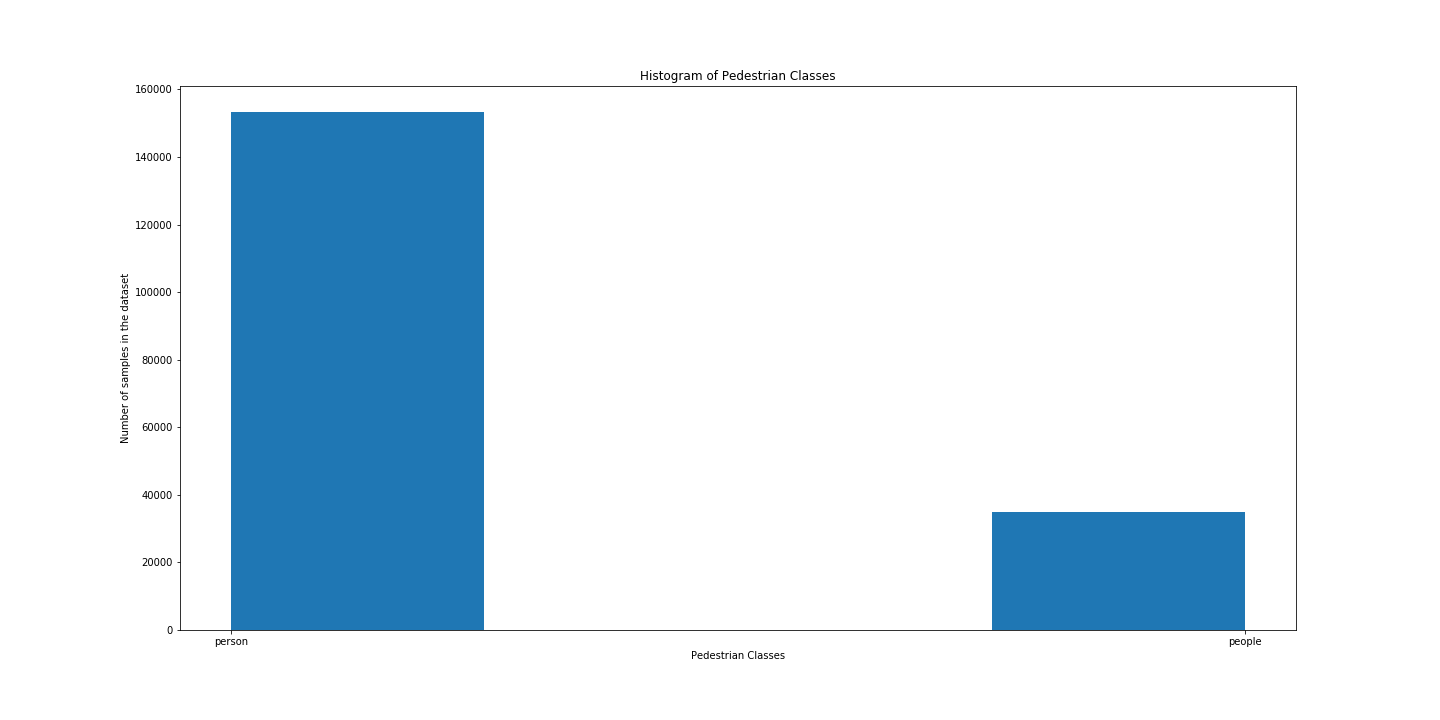
\includegraphics[scale=0.4]{classid_distribution1_2}
\begin{center}
\caption{Class 'person' and 'people' distribution}
\end{center}
\end{figure}

As per \cite{walk2010new}, unoccluded pedestrians with 50-pixel-or-taller are considered , as they are not clear. For simplicity purpose below data are discarded from the training set.
\begin{itemize}
	\item Class label with \textit{people}, \textit{person-fa}, \textit{person?}
	\item occluded \textit{person} label
	\item images below 50 pixel in height
	\item images below 5 pixel in width
\end{itemize}

After the above mentioned clean up, our training data contains total 48194 number of BB with person as a label in 26902 unique frames and sample data looks as below:
\begin{center}
\texttt{  \\
frame,xmin,xmax,ymin,ymax,class\textunderscore id \\
set00\textunderscore V000\textunderscore 1213.png,573,591,169,211,1 \\
set00\textunderscore V000\textunderscore 1213.png,473,484,170,193,1 \\
set00\textunderscore V000\textunderscore 166.png,406,418,164,187,1 \\
set00\textunderscore V000\textunderscore 166.png,435,442,167,181,1 \\
set00\textunderscore V000\textunderscore 166.png,233,241,120,134,1 \\
set00\textunderscore V000\textunderscore 744.png,564,588,153,218,1 \\
set00\textunderscore V000\textunderscore 744.png,565,587,173,206,1 \\
set00\textunderscore V000\textunderscore 654.png,406,417,162,194,1 \\
}
\end{center}

During the training an NVIDIA GeForce GTX 1080 GPU with 8GB of video memory was used, while using a validation data size equals to standard 10\% of training data, the training time was equals to unusable, as training of a single epoch was taking nearly ~30-40 hours. The experiment was run on a shared Linux server hosted within the University Network and the computing resource was shared with other students. Keeping this in view, i decided to reduce the size of the validation data set size to great extent and get an approximate impression about the model's training efficiency. Below table show the training and validation data partition.

\begin {table}[H]
\begin{center}
 \begin{tabular}{||c c c||}
 \hline
 Data Set & Bounding Box & Frames\\ [0.8ex] 
 \hline\hline
 Training & 47194 & 26280 \\
 \hline
 Validation & 1000 & 622 \\
 \hline
 Total & 48194 & 26902 \\
 \hline
\end{tabular}
\caption{Training and Validation sample numbers}
\end{center}
\end {table}

\cite{dollar2009pedestrian} defines pedestrians with 80 pixels or taller as in the near scale and 30 pixel or less
are in the far scale and rest in the medium scale. Most pedestrians are observed in medium scale. A person with 1.8m tall is 1.5s away from the vehicle for the mentioned set up and speed of 55km\/h. \cite{dollar2011pedestrian} shows that average aspect ratio \textit{$w \approx 0.41h$}. After above mentioned cleaning steps, a re calculation for the aspect ration distribution shows, it does not vary much from the original distribution, as shown below.

\begin{figure}[H]
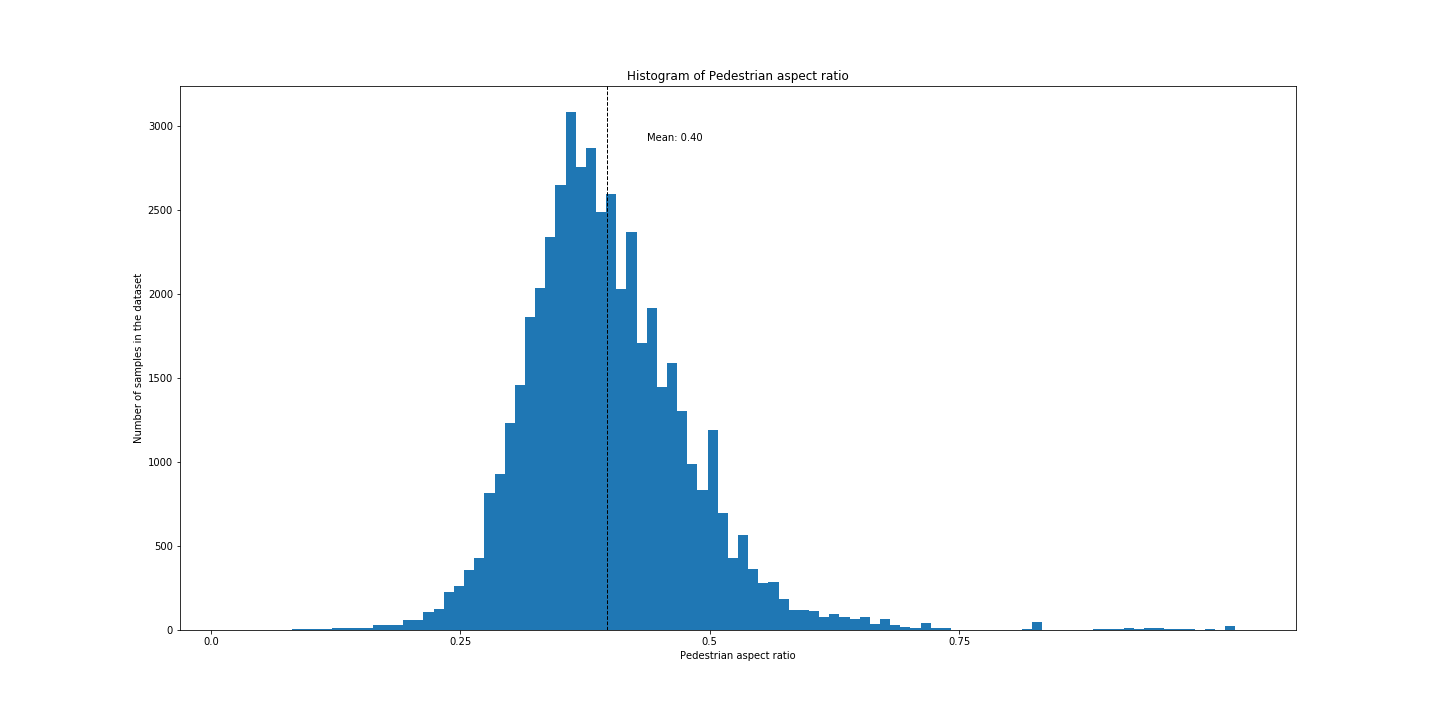
\includegraphics[scale=0.4]{aspect_ratio_distribution}
\begin{center}
\caption{Pedestrian aspect ratio distribution}
\end{center}
\end{figure}

\section{Training }
As SSD has predictors at multiple level, before the model training step, a pre-processing step is required where proposed BBs are generated and compared with the ground truth and depending on IoU threshold, certain prior BBs are considered and encoded for the training purpose. There are several parameters play a role in generating bounding boxes and some of critical parameters used are given below.

\subsection{Framework parameters}

\begin {table}[H]
\begin{center}
 \begin{tabular}{||c c||} 
 \hline
 Param. Name & Value\\ [0.8ex] 
 \hline\hline
 img\textunderscore  height & 480 \\ 
 \hline
 img\textunderscore  width & 640 \\
 \hline
 img\textunderscore  channels & 3 \\
 \hline
 n\textunderscore  classes & 1 \\
 \hline
 scales & $[0.08, 0.16, 0.32, 0.64, 0.96]$ \\
 \hline
\end{tabular}
\caption{SSD framework parameters}
\end{center}
\end{table}

\subsection{Model parameters}
\textbf{Model Architecture:}
SSD model consists of convolutional feature layers and some convolutional predictor layers that take input from different feature layers, making the model fully convolutional. In the presented model, 7 convolutional layers and 4 predictors layers are used. These 4 convolutional predictors layers take input from layers 4, 5, 6, and 7 respectively. convnet with was used for modeling using keras \footnote{Keras is a high-level neural networks API, written in Python and capable of running on top of TensorFlow, CNTK, or Theano.}. The model is created and initialised with Keras API Sequential (). 

\subsection{Hyper Parameters}

\section{Testing}

\subsection{Graphs and results}

After training for 10 epochs the training error gradually reduces and the validation error revolves around training error as shown in the below graph. As the training of single epoch takes significant time the statistics were taken with small epochs.

\begin{figure}[H]
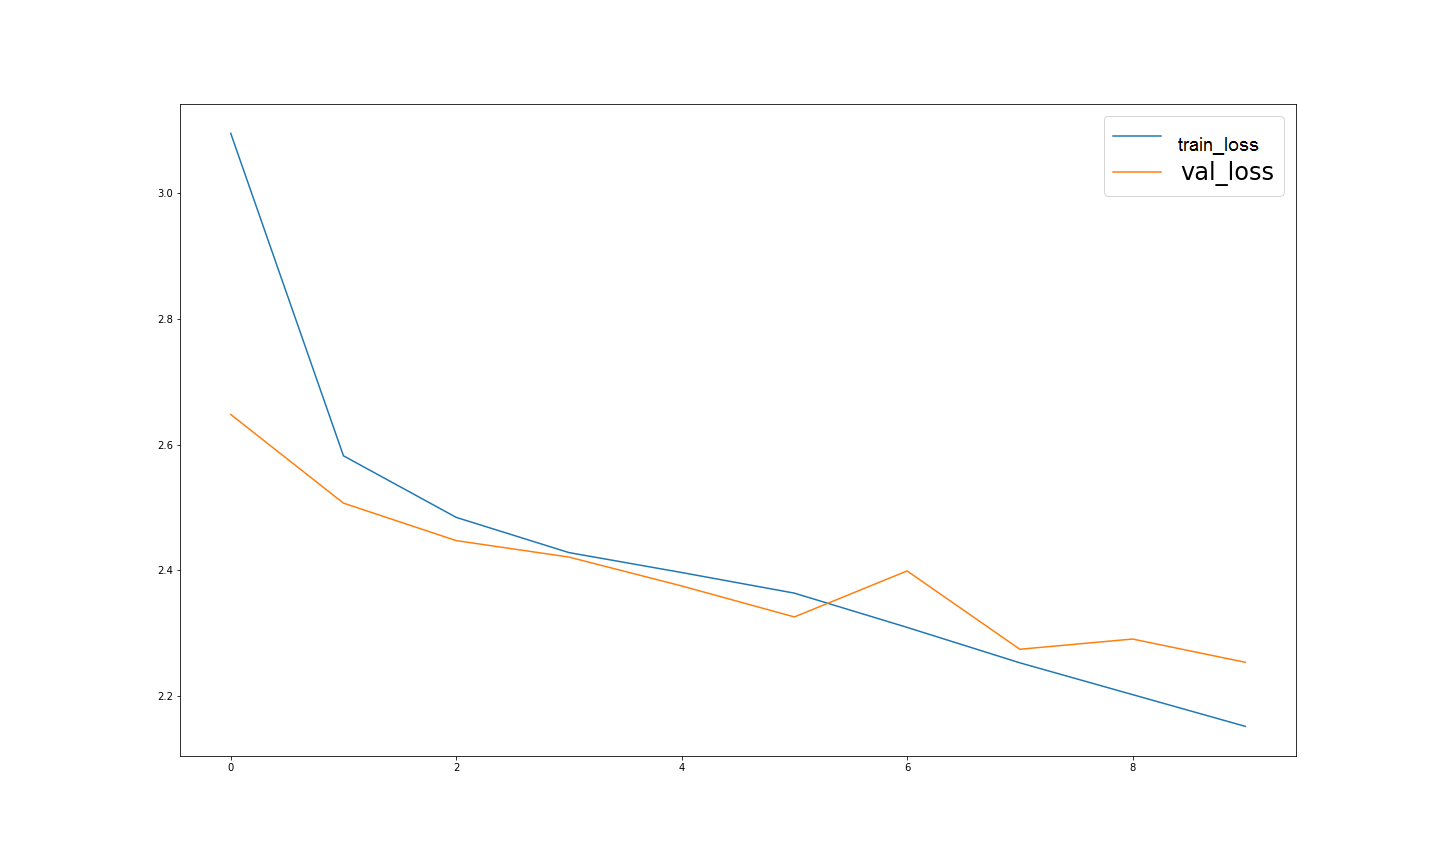
\includegraphics[scale=0.4]{conf0_loss-val_loss_0_10epochs}
\begin{center}
\caption{Training and Validation error after 10 epochs}
\end{center}
\end{figure}
As the training error has not converged after 10 epochs it was decided to training for another 10 epoch and the graph as follows.

\begin{figure}[H]
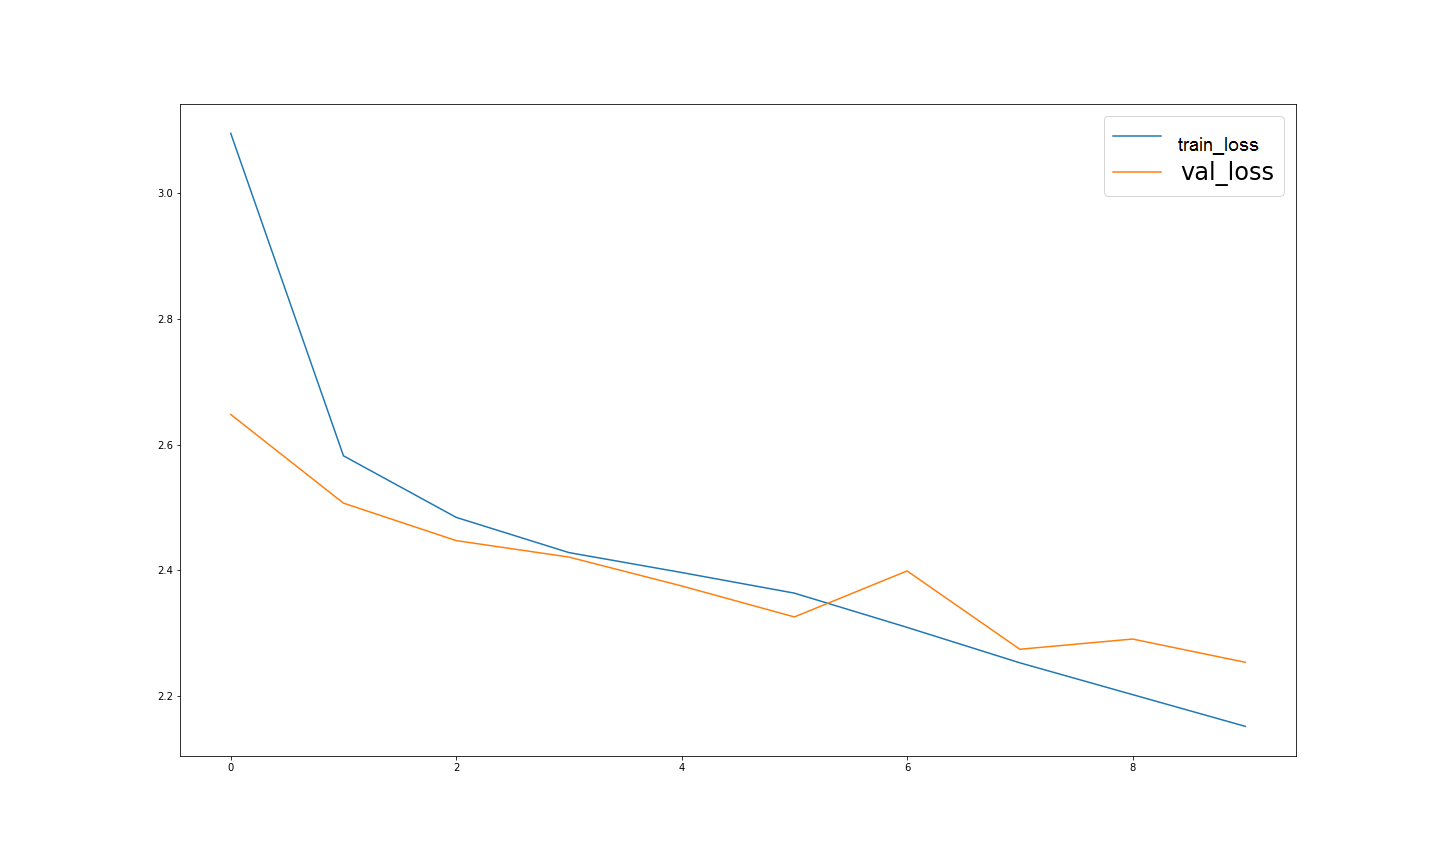
\includegraphics[scale=0.4]{conf0_loss-val_loss_0_10epochs}
\begin{center}
\caption{Training and Validation error after 10 epochs}
\end{center}
\end{figure}

\textbf{Validation:}

\newpara
\textbf{Observation:} While using SSD7, i observed that the algorithm is very sensitive to the list of aspect ratios for the anchor boxes. To begin with, the values for aspect\textunderscore ratios = $[0.5, 1.0, 2.0]$ were used and that lead to very poor result in the evaluation phase. After modifying aspect\textunderscore ratios = $[0.1, 0.2, 0.33, 0.413, 0.418, 0.5, 0.6, 0.7, 0.8, 1.0]$, recorded accuracy as below table.
From Caltech data set video set 06 - 10 was used as test data. The bounding box, label are extracted into labels\textunderscore test\textunderscore full.csv using a python script. labels\textunderscore test\textunderscore full.csv consists of total 154436 records. After removing occluded and other classes except person, remaining number of records were 73218 , where the unique number of images are 42910. After discarding records with less than 50 pixel for height or 5 pixel for width we are left with 29620. Randomly chosen 1000 records were taken for test purpose for recording the \textit{mAP}. These test 1000 records consists of unique 902 images.

\begin{table}[H]
\begin{center}
 \begin{tabular}{||c c c||} 
 \hline
 No. epoch & mAP & fps\\ [0.8ex] 
 \hline\hline
 10 & 0.661 & 10.22\\ 
 \hline
 20  & TBD & TBD \\
\hline
 20  & TBD & TBD \\
 \hline
\end{tabular}
\caption{Average Precision and fps with number of epochs}
\end{center}
\end{table}

\section{JAAD Dataset}

JAAD \cite{rasouli2017agreeing} is a publicly available large scale data set that includes data for pedestrian detection with behavioral and contextual information. It contains 346 video clips of pedestrian data that includes occlusion label, temporal correlation, behavioral aspect, contextual information weather related data. Rasouli et al. provided a supporting GitHub code for easier interaction with JAAD data. The videos can be downloaded by running the script \colorbox{lightgray}{download\textunderscore clips.sh}. The video clips are downloaded into JAAD\textunderscore clips and the clips are named as below.\\
\colorbox{lightgray} {JAAD\textunderscore clips/video\textunderscore  0001.mp4} \\
\colorbox{lightgray} {JAAD\textunderscore clips/video\textunderscore  0002.mp4}

Using \colorbox{lightgray}{split\textunderscore clips\textunderscore to\textunderscore .sh} the frames are extracted to corresponding video id directory with in a floder called \textit{images} \\
\begin{center}
\colorbox{lightgray} {images/video\textunderscore  0001/0000.png} \\
\colorbox{lightgray} {images/video\textunderscore  0001/0001.png} \\
\colorbox{lightgray} {....}
\end{center}

In JAAD annotations are divided into 5 groups:
\begin{itemize}
	\item Annotations: Information about pedestrian bounding box, occlusion information, activities. These annotations are one per frame per label.
	\item Attribute: Contains information regarding pedestrian’s crossing points, crossing characteristics. These annotations are one per pedestrian.
	\item Appearance: Information regarding pedestrian pose, clothing, objects they carry. These information are one per frame per pedestrian.
	\item Traffic: Includes information about traffic signs, traffic light for each frame.
	\item Vehicle: Per frame vehicle speed information e.g moving fast, speeding up.
\end{itemize}


The early work includes prediction of road users behavior by employing dynamic factors e.g trajectory prediction, velocity prediction or predicting final goal of the pedestrian. Recently behavioral aspect such as awareness by estimating head orientation along with other contextual information such as sign, weather condition, visibility and individual characteristics of the pedestrian such as things he carry, age and sex, size of the group he is associated with influence crossing behavior.

TODO:  pedestrian to identify the pedestrians with behavioral tags (i.e. the ones demonstrating the intention of crossing or located close to the curb). 
Occlusion information is provided in the form of tags for
each bounding box: partial occlusion (between 25\% and 75\%
visible) and full occlusion (less than 25\% visible).
 654 unique pedestrian samples (out of 2.2k samples) with behavioral tags in the
dataset. 
The
pedestrians\' actions are categorized into 3 groups: Precondition- this refers to the state of the pedestrian prior to crossing and can be either standing, moving slow or fast. Attention- the way the pedestrian becomes aware of the approaching vehicle. These actions, depending on their duration, are looking ( > 1s) or glancing ($\leq$ 1s). Response- this
includes the behaviors that pedestrians exhibit in response
to the action of the approaching vehicle, namely, stop, clear path, slow down, speed up, hand gesture and nod.

Weakly supervised learning!
Sigmoid cross entropy vs  softmax
batch normalization